\chapter{A New Economy for An Old Problem}
\label{neweconomy}

In this section, we provide an overview of current stubble management practices and the state-of-the-art Pineapple Leaves (PAL) valorisation options in Costa Rica. The information provided in this section is based on academic and grey literature and findings from interviews and observation. The present documentation serves to analyse the potential business models for the PAL and their corresponding benefits and limitations. 

\begin{figure}[H]
\caption{Structure of pineapple plant}
\label{pineappleStructure}
\centering
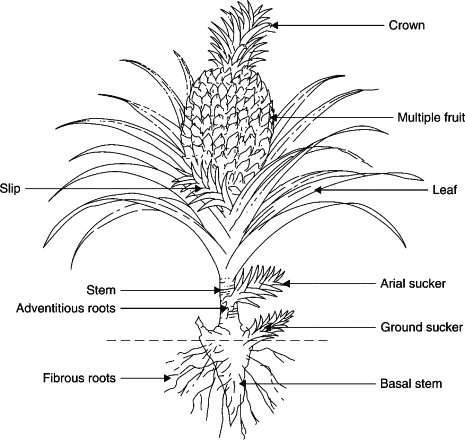
\includegraphics[width=6cm]{fig/pineappleStructure.png}

\scriptsize Source: \cite{hassan2011pineapple}
\end{figure}

The main parts of a pineapple plant are the crown, the fruit, the slips, a short and thick stem, two suckers, and a rosette of long (0.50–1.8 m), narrow, fibrous leaves. The structure of the pineapple is depicted in figure \ref{pineappleStructure}. The pineapple production cycle, from plantation to harvest, lasts between 12 and 18 months. In Costa Rica, the production cycle is usually profitable only for two harvests \citep{ingwersen2012life, magHarvest, zhang2016phenological}. After the last harvest, the ratoons from the plants are harvested to use as seeds for new plantations. At this point, the plantation, usually managed per hectare, needs to be taken down, The plants, now considered stubble, or organic residues, need to be handled to make room for a new plantation.

\section{Current practices of pineapple stubble management}

The fast increase in pineapple demand in the 2010s created an urgent need to accelerate the pineapple production cycle. To avoid the propagation of the stable fly and shorten the time between harvest and new plantation, practices to rapidly manage the stubble were implemented. practices vary depending on the producer's size and earnings, on how rapidly the field needs to be ready for a new plantation, and on the knowledge and ability of the producer to implement available management practices.

The two most common ways to treat the stubble are green management (\textit{en verde}) and dry (\textit{en seco}) management. Green management involves harrowing the stubble with mechanical equipment (\textit{rastra}) directly in the field to be incorporated into the soil. Dry management requires drying the plant with herbicides, then burning it with fire, and finally incorporating it into the soil \citep{pineChaverri2022}. Although green management does not require agrochemicals, producers more often use dry management because it is more cost-effective \citep{hernandez2018impacto}. 

Three other practices are less widely used in Costa Rica today. These are burying (in a pit), piling up in a mountain of stubble, and decomposition through decomposers. Burying and piling up are costly options that require access to additional land to dig and bury or to accumulate the stubble. The use of these practices, which allows for an immediate new plantation, is identified in plantations managed by large companies with access to machinery and land. The use of decomposers, although mentioned in a stubble management handbook published by an agency of the Ministry of Agriculture of Costa Rica \citep{gonzalezMAG2012}, is seldom implemented and it is nowadays only used by small and medium-sized producers. Management with decomposers is beneficial for the environment as it does not require agrochemicals, but its implementation must be rigorously monitored as, otherwise, it can be ineffective in avoiding the propagation of the stable fly. The use of decomposers is accompanied with harrowing and, if implemented correctly, can considerably accelerate the decomposition of stubble. 

Regardless of the type of practice used, managing the stubble takes time and costs money to the producer. There is no perfect solution to accelerate the decomposition of organic matter and control the propagation of stable flies. Should the fly not be a problem for close-by ranchers and communities, the stubble could theoretically be left on the ground until naturally decomposed, but producers also prefer to accelerate the decomposition and, consequently, the production cycle. Perhaps the only advantage of managing the stubble at the field is the return of nutrients to the soil during stubble decomposition \citep{liu2013effects}.

\section{Potential ways of valorising PAL}
\label{valoriseOptions}

Since the management of stubble in the field generates environmental and financial costs, producers and researchers have developed ideas to valorise the residues of pineapple cultivation. In this section, we focus only on the valorisation options that are being developed or considered in Costa Rica. For a summary of the many PAL valorisation options, see \cite{aili2021recent}, and for a review of agro-industrial biowaste valorisation in Costa Rica, see \cite{eixenberger2022tropical}. The options to valorise PAL in Costa Rica can be divided into three categories: energy generation, feed production, and biobased product production, the latter having two main subcategories, textiles, and other biobased products. Below, we describe these options, their stage of development in Costa Rica, and considerations regarding their demand and regulation. 

The energy production from PAL follows a similar process to that of other biomasses, and its production requirements and potential have been studied extensively. \cite{chen2020production} developed a simple process that converts one hectare of PAL into 2.1 tonnes of bioethanol, 1.55 tonnes of spent yeast biomass, and 11.65 tonnes of dry fibrous material. They concluded that the amount of bioethanol that can potentially be produced from PAL would replace approximately 8.5\% of the fuel consumption for transportation in Costa Rica. Despite the study by \citeauthor{chen2020production}, no PAL-based biorefinery process has been implemented in Costa Rica at any scale. There is no well-defined legal framework to produce biofuels in Costa Rica. As described in the 2015-2030 National Energy Plan, the main barrier to introducing biofuel blending is the nonexistence of a public-private strategy. The private sector has the capacity to produce biofuels, but RECOPE, the national oil refinery, is the one responsible for establishing the parameters of the mixture and producing the blending \citep{planClimaCR}. Regarding the demand for fuel blending, this will depend on the price of fossil and biofuels and the policies on biofuels, such as the EU \citeauthor{Directivebiofuels}. The Costa Rican government has mentioned that it would work to introduce a biofuel policy \citep{ChavesEtanol}. Producing bioethanol is economically viable only at an exceptionally large scale, and implementing this solution for PAL poses a logistical challenge and requires large initial investments. For more studies on PAL-based biorefinery processes to produce biofuels in different places and at different scales, see \cite{murcia2022biorefinery, saini2022valorization, silva2020second, mund2021cellulose}.

Biogas is another energy production alternative that is often discussed in the literature. \cite{arce2014determinacion} provides a detailed report on an experiment conducted to determine the capacity of biogas generation with PAL in Costa Rica. More details on the scalability at a national scale drawn from their results are discussed in \cref{costsch4}. \cite{kohlmann2015, barz2019agricultural} provide a life cycle eco-efficiency study of biogas production from pineapple and other agricultural residues in tropical and subtropical regions and estimate a reduction of more than 1-tonne \ch{CO2}-eq \si{\per\hectare} for PAL in Costa Rica. Nonetheless, they use an average transportation distance of 20 km which is an underestimate compared to our calculations. In 2017, a pilot project to produce biogas from PAL was done in Upala (NW of Costa Rica) \citep{iceValle}. Apart from the studies mentioned here and pilot projects briefly described in news articles, there is no information on previous projects or active PAL-based biogas plants. However, there are several studies on the production of biogas with other pineapple waste (peel and core) \cite{aili2021recent}. Biogas can be used in two ways, either compressing it to fuel vehicles or as a replacement for natural gas, in which case it can be used for heating and electricity generation. Compressing it requires a lot of energy, so biogas is not considered a feasible alternative to fossil fuels. Although heating is not required in the Costa Rican climate, the electricity produced from biogas is an attractive application of PAL. More than 95\% of Costa Rica's electrical energy is derived from renewable energy sources \cite{iceEnergia}, and the privately generated electricity must be sold to the national grid controlled by the Costa Rican government-run Institute of Electricity (ICE). The challenge when producing biogas for electricity generation is therefore to make it cost-competitive relative to the already available electricity mix.
 
The PAL fibre (PALF), which yields around 2\% of the fresh leaf, can be processed into several products, such as textiles, paper, rope, and composite materials. The study of different applications of PALF is extensive. \cite{rafiqah2020effect} provide exhaustive documentation of extraction processes, properties, comparisons with other natural fibres, and applications of PALF. A recent summary of the possible applications of PALF composites, such as in the automobile or construction industries, and an analysis of the PALF mechanical and thermal strength can be found in \cite{jain2022pineapple}. The existing PALF extraction methods and the chemical modification to produce textiles (woven, non-woven, and knitted fabrics) from PALF are described in \cite{jose2016overview}. A feasibility analysis of using PALF for paper production is provided by \cite{sibaly2017production}. Studies of PALF applications in Costa Rica can be found mainly in the form of dissertations (see, e.g., \cite{tecDissertation, cuerdaUCR, NanofibriUNA}. There have also been small ventures to manufacture fibre from PAL in Costa Rica, but to this day there are no PALF manufacturing companies in the country. Because current technology to extract the fibre from pineapple leaves is labour-intensive, establishing a large-scale PALF extraction operation is not feasible. The demand for PALF-based products already starts in the pineapple industry; the material used to produce packaging solutions for transporting pineapples, such as cardboard boxes, pallets, and edge protectors, can be partly replaced with PALF composites. Moreover, rope used in the pineapple fields can be replaced with rope made with PALF. Finally, the potential to produce biodegradable alternatives to plastics with PALF is of interest to a country that is trying to phase out single-use plastics, as demonstrated by the 	
plastic bag legislation \cite{LeyN9786} and the single-use plastic ban in national parks \cite{sinacPlastic}, with effect from 2019 and 2021, respectively. 

The easiest PAL valorisation option, due to its relatively constant demand and its simple process, is animal feed. Fresh, ensiled, or converted into pellets, PAL can be used as a substitute for part of ruminants' diets. \cite{buliah2019production} study the properties of PAL-made pellets for feeding dairy cows. \cite{lopez2009caracteristicas} determined the nutritional value and fermentative parameters of pineapple leaves, suckers, and stems before and after ensilaged. In Costa Rica, the crown of pineapples is usually given for free to ranchers who complement their cattle's diet with it. The only large-scale operation of PAL valorisation in the country was identified in a pineapple production company that collects PAL to produce and sell silaged PAL. The diet of dairy cattle often consists of forage and grain (concentrates), and this PAL cannot completely substitute it, but it can serve as a complement, especially in the dry season. 

\section{Extraction from the field}

To valorise the PAL, this first needs to be extracted from the field. Extracting the plant requires two basic steps, (1) cutting or pulling the plant from the ground and (2) collecting the plants in trucks to transport them to a facility. In \cref{FLPchapt4}, we discuss the relevant aspects related to the transportation of PAL through the national road network. The fields where pineapple grows, characterised by hilly and wet terrain, and the presence of trenches to allow rainwater to flow, make the manoeuvring of machinery difficult. Several agricultural machines developed for other purposes, crops and terrains have been tested in pineapple plantations to extract and collect PAL, but the results have not been satisfactory (see, e.g., \cite{monniAnanas}). As for the collection of PAL, the large above-ground volume of pineapple plants requires the shredding of the leaves in the field or, if desired for fibre extraction, transporting large dimensional weights of leaves. 

There seems to be a consensus that the disadvantages of extracting the stem and roots of the pineapple outweigh the benefits. This part of the pineapple is contaminated with soil and would need to be cleaned prior to further processing. Moreover, extracting the soil adds to the weight that needs to be transported and contributes to soil depletion. Thus, most extraction ideas, either by machine or manually, contemplate the cutting of the leave above the aerial sucker (see \cref{pineappleStructure}). To this day, the only implementation of a large-scale PAL extraction operation consists of a truck with lateral arms, similar to how pineapple harvesters work, in which farm labourers need to place the previously cut plant to be rolled by a conveyer into the truck. This solution is still far from a fully mechanised operation.

A mechanised solution to extract the PAL has been envisioned mainly in two ways. First, a large vehicle capable of driving through the field, cutting and collecting the PAL has been prototyped. The problem with this type of vehicle is the required horsepower, the pressure placed on the ground, and the small capacity to manoeuvre on difficult terrain. The second idea consists of a tyre or track tractor capable of driving above the fields, to which a cutter would be attached. This second solution is practical for the type of terrain, but it requires a second vehicle to collect the PAL.

